% Template for ICASSP-2013 paper; to be used with:
%          spconf.sty  - ICASSP/ICIP LaTeX style file, and
%          IEEEbib.bst - IEEE bibliography style file.
% --------------------------------------------------------------------------
\documentclass{article}
\usepackage{spconf,amsmath,graphicx}
\usepackage{graphicx}
\usepackage{cite}
\usepackage{url}
\usepackage{hyperref}
\usepackage{cleveref}
\usepackage{booktabs}
\usepackage{brian}

% Title.
% ------
\title{Learning to segment songs with ordinal linear discriminant analysis}
%
% Single address.
% ---------------
% \name{Author Names\thanks{Thanks to XYZ agency for funding.}}
% \address{Author Affiliations}
%
% For example:
% ------------
%\address{School\\
%   Department\\
%   Address}
%
% Two addresses (uncomment and modify for two-address case).
% ----------------------------------------------------------
\twoauthors%
 {Brian McFee}{ Center for Jazz Studies\\
      Columbia University\\
  \texttt{brm2132@columbia.edu}}%
 {Daniel P.W. Ellis}{
  LabROSA, Department of Electrical Engineering\\
      Columbia University\\
  \texttt{dpwe@columbia.edu}}
%
\begin{document}
%\ninept
%
\maketitle
%
\begin{abstract}
Segmentation is sweet
\end{abstract}
%
\begin{keywords}
Music information retrieval, automatic segmentation, supervised learning
\end{keywords}
%
\section{Introduction}
\label{sec:intro}

\subsection{Our contributions}

\section{Related work}
\label{sec:related}

\section{Evaluation}
\label{sec:eval}

\subsection{Implementation}

\subsection{Results}
\label{sec:results}

\begin{table*}[t]
\centering
\caption{Segmentation performance on Beatles-ISO. OLDA was trained on the SALAMI-free corpus.\label{tab:results:beatles}}
\begin{tabular}{lrrrrrrrrrrrr}
\toprule%
Algorithm   &   $P_{0.5s}$ & $R_{0.5s}$ & $F_{0.5s}$ & $P_{3s}$     & $R_{3s}$  & $F_{3s}$   & $S_O$ & $S_U$ & $S_F$ & $P_L$& $R_L$& $F_L$\\
\hline
Native      &   \textbf{0.446} & 0.390 & 0.408 & 0.704   & 0.603 & 0.640 & \textbf{0.842} & 0.755 & 0.791 & \textbf{0.780} & 0.613 & 0.668\\
OLDA        &   0.438 & \textbf{0.447} & \textbf{0.434} & 0.685   & 0.680 & 0.670 & 0.828 & 0.808 & 0.813 & 0.744 & 0.686 & 0.694\\
\hline
SMGA~\hfill\cite{serra2012unsupervised}
            &   0.358 & 0.393 & 0.370 & \textbf{0.769}   & \textbf{0.808} & \textbf{0.780} & 0.811 & \textbf{0.858} & \textbf{0.829} & 0.702 & \textbf{0.798} &
            \textbf{0.729}\\
\bottomrule%
\end{tabular}
\end{table*}

\begin{table*}[t]
\centering
\caption{Segmentation performance on SALAMI-free. OLDA was trained on the Beatles-ISO corpus.\label{tab:results:salami}}
\begin{tabular}{lrrrrrrrrrrrr}
\toprule%
Algorithm       &   $P_{0.5s}$ & $R_{0.5s}$ & $F_{0.5s}$ & $P_{3s}$     & $R_{3s}$   & $F_{3s}$   & $S_O$ & $S_U$ & $S_F$ & $P_L$& $R_L$& $F_L$\\
\hline
Native  & 0.400 & 0.364 & 0.372 & \textbf{0.610} & 0.557 & 0.570 & \textbf{0.812} & 0.795 & 0.794 & \textbf{0.666} & 0.652 & 0.626\\
OLDA    & \textbf{0.406} & \textbf{0.407} & \textbf{0.396} & \textbf{0.610} & 0.611 & \textbf{0.597} & 0.804 & 0.829 & \textbf{0.808} & 0.640 & 0.707 & \textbf{0.640}\\
\hline
SMGA~\hfill\cite{serra2012unsupervised}
        & 0.209 & 0.360 & 0.256 & 0.512 & \textbf{0.733} & 0.589 & 0.714 & \textbf{0.895} & 0.786 & 0.448 & \textbf{0.822} & 0.550\\
% C-NMF~\cite{nieto2013convex}& -- & -- & -- & 0.430 & 0.523 & 0.451 & 0.506 & 0.443 & -- & 0.440 & 0.810 & 0.531\\
% SI-PLCA~\cite{weiss2011unsupervised} & -- & -- & -- & 0.195 & 0.461 & 0.256 &  0.442 & 0.514 & -- & 0.558 & 0.521 & 0.513\\
C-NMF~\hfill\cite{nieto2013convex}            
        & -- & -- & -- & 0.430 & 0.523 & 0.451 & -- & -- & -- & -- & -- & -- \\
SI-PLCA~\hfill\cite{weiss2011unsupervised}    
        & -- & -- & -- & 0.195 & 0.461 & 0.256 & -- & -- & -- & -- & -- & -- \\  
\bottomrule%
\end{tabular}
\end{table*}

\begin{figure*}[t]
\centering%
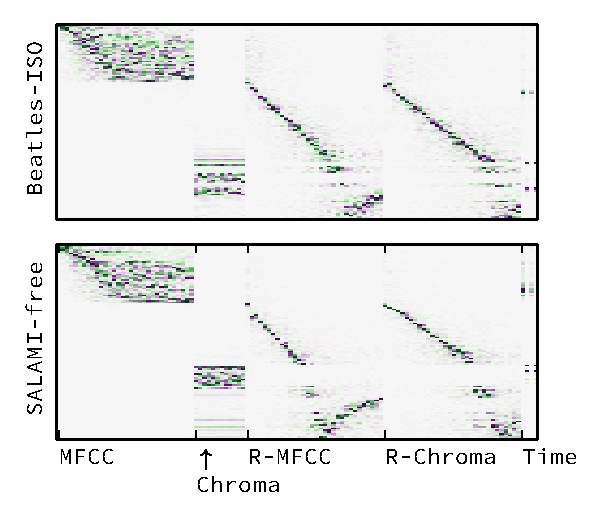
\includegraphics[width=0.95\textwidth]{figs/w}%
\caption{OLDA transformations $W\trans$ learned on Beatles-ISO and SALAMI-free. Each row corresponds to a projection
direction, and the rows are ordered by decreasing importance from top to bottom.\label{fig:w}}
\end{figure*}

\section{Conclusion}
\label{sec:conclusion}


\bibliographystyle{IEEEbib}
\bibliography{refs}

\end{document}
